\documentclass[10pt]{article}
 
\usepackage[margin=1.5cm]{geometry} 
\usepackage{amsmath,amsthm,amssymb}
\usepackage{polski}
\usepackage[utf8]{inputenc}
\usepackage{siunitx}
\usepackage{graphicx}
\usepackage{comment}
\usepackage[font=scriptsize]{caption}
\usepackage{subcaption} 
\usepackage{array}
\usepackage{hyperref}
\usepackage[section]{placeins}

\newcolumntype{C}[1]{>{\centering\let\newline\\\arraybackslash\hspace{0pt}}m{#1}}

\newenvironment{theorem}[2][Twierdzenie]{\begin{trivlist}
\item[\hskip \labelsep {\bfseries #1}\hskip \labelsep {\bfseries #2.}]}{\end{trivlist}}
\newenvironment{question}[2][Pytanie]{\begin{trivlist}
\item[\hskip \labelsep {\bfseries #1}\hskip \labelsep {\bfseries #2.}]}{\end{trivlist}}
\newenvironment{hypothesis}[2][Hipoteza]{\begin{trivlist}
\item[\hskip \labelsep {\bfseries #1}\hskip \labelsep {\bfseries #2.}]}{\end{trivlist}}
\newenvironment{lemma}[2][Lemat]{\begin{trivlist}
\item[\hskip \labelsep {\bfseries #1}\hskip \labelsep {\bfseries #2.}]}{\end{trivlist}}
\newenvironment{exercise}[2][Ćwiczenie]{\begin{trivlist}
\item[\hskip \labelsep {\bfseries #1}\hskip \labelsep {\bfseries #2.}]}{\end{trivlist}}
\newenvironment{reflection}[2][Uwaga]{\begin{trivlist}
\item[\hskip \labelsep {\bfseries #1}\hskip \labelsep {\bfseries #2.}]}{\end{trivlist}}
\newenvironment{proposition}[2][Założenie]{\begin{trivlist}
\item[\hskip \labelsep {\bfseries #1}\hskip \labelsep {\bfseries #2.}]}{\end{trivlist}}
\newenvironment{corollary}[2][Wniosek]{\begin{trivlist}
\item[\hskip \labelsep {\bfseries #1}\hskip \labelsep {\bfseries #2.}]}{\end{trivlist}}
\newcommand{\expnumber}[2]{{#1}\mathrm{e}{#2}}

\begin{document}
\title{Rozwiązywanie 3-SAT - algorytm DPLL vs strategie ewolucyjne}
\author{Grams, Stanisław (251000)\\ MFI UG\\Inteligencja Obliczeniowa}

\maketitle
\section {Wstęp}
Tematem projektu jest porównanie wydajności jednego algorytmu i dwóch heurystyk pozwalających na rozwiązywanie problemów 3-SAT.
Problem spełnialności (SAT) jest fundamentalnym problemem NP-zupełnym - czyli takim do którego każdy problem z klasy NP można zredukować w czasie wielmianowym.
Odpowiednio szybki algorytm SAT mógłby zostać zastosowany m.in. w planowaniu w czasie rzeczywistym, obliczeniach charakterystycznych dla elektroniki czy astronautyki, gdzie znaleźć należy optymalne rozwiązanie problemu klasy NP-zupełnego.

\subsection{Narzędzia}
Programy zaimplementowano od podstaw w języku \textit{Python 3}\footnote{\url{https://www.python.org/}} oraz użyto nastepujących bibliotek zewnętrznych:
\begin{itemize}
  \item matplotlib\footnote{\url{https://matplotlib.org/}} - biblioteka pozwalająca na stworzenie wykresów z poziomu pythona
  \item pandas\footnote{\url{https://pandas.pydata.org/}} - biblioteka pozwalająca na łatwą kontrolę nad plikami csv
\end{itemize}

\subsection{Dane}
Dane wejściowe pochodzą ze strony internetowej \textit{cs.ubc.ca/~hoos/SATLIB/benchm.html}\footnote{\url{https://www.cs.ubc.ca/~hoos/SATLIB/benchm.html}} - agregującej dane wejściowe dla problemów typu SAT.
Plik importowany przez program zdefiniowany jest w specyficznym dla problemów SAT formacie DIMACS\footnote{\url{https://logic.pdmi.ras.ru/~basolver/dimacs.html}}.

\subsection{Zaimplementowane oraz użyte algorytmy}
\begin{itemize}
  \item (\textbf{DPLL}): Współczesny algorytm DPLL\footnote{\url{https://en.wikipedia.org/wiki/DPLL_algorithm}}\footnote{\url{https://www.win.tue.nl/~jschmalt/teaching/2IMF20/BMC-lecture_slides_SAT.pdf}}
  \item (\textbf{SGA}): Standardowy algorytm genetyczny z możliwością elityzmu\footnote{\url{https://pl.wikipedia.org/wiki/Algorytm_genetyczny}}
	\item (\textbf{IAGA}): Adaptacyjny algorytm genetyczny zaimplementowany na podstawie publikacji\footnote{\url{https://www.atlantis-press.com/journals/ijcis/25888772/view&sa=D&ust=1579988144931000}}
\end{itemize}
Testy zostały wykonane dla zmiennych $L=20 .. 90$ i klauzul $M=10 .. 449$.\\
\section{\textbf{SGA}: Standardowy algorytm genetyczny}
Zaimplementowano standardowy algorytm genetyczny oraz przeprowadzono testy. Zadziwiająco, dla dowolnej liczby zmiennych oraz klauzul najlepszymi okazały się poniższe parametry, oraz to własnie ich użyto w celu dalszej ewaluacji rozwiązania.

\begin{center}
		\begin{tabular}{|C{5cm}|C{5cm}|}
			\hline
			\textbf{nazwa współczynnika} & \textbf{wartość} \\ \hline
			{crossover rate} & 0.90\\ \hline
			{mutation rate} & 0.08\\  \hline
      {population size} & 50 \\ \hline
      {generations} & 1000 \\ \hline
      {elitism} & True \\ \hline
		\end{tabular}
\end{center}

Funkcję fitness w przypadku \textbf{obu algorytmów genetycznych} można określić poniższym wzorem:
\begin{center}
  $F = \frac{S}{C}$
\end{center}
gdzie S oznacza ilość spełnionych klauzul przez chromosom, a C oznacza ilość wszystkich klauzul.
\section{\textbf{IAGA}: Improved Adaptive Genetic Algorithm}
Głównymi róznicami między typowym algorytmem genetycznym rozwiązującym problemy 3-SAT a zaimplementowanym ulepszonym, adaptywnym algorytmem genetycznym wynikają wprost z nazwy publikacji, w której się ukazał \textit{An Improved Adaptive Genetic Algorithm for Solving 3-SAT Problems Based on Effective Restart and Greedy Strategy}.
\begin{figure}[h]
\centering
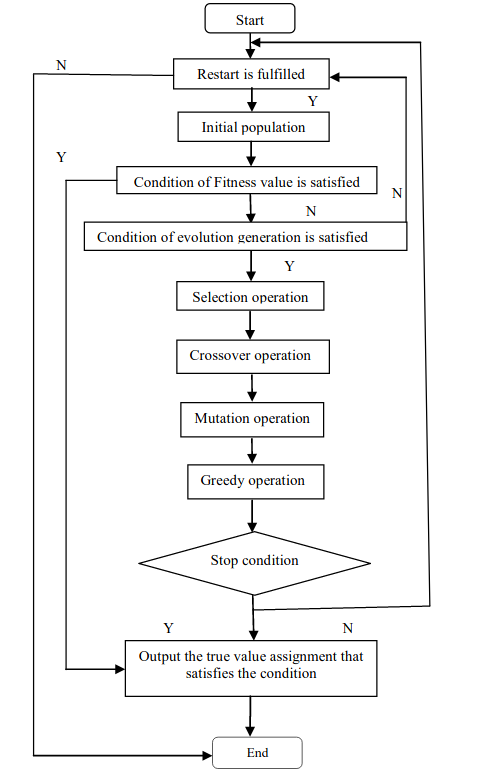
\includegraphics[scale=0.5]{img/iaga.png} \\
Flow chart heurystyki \textbf{IAGA}
\end{figure}

Heurystyka ta wykazuje się trzema głównymi zmianami w stosunku do standardowego algorytmu genetycznego:
\begin{enumerate}
  \item adaptywnie w trakcie ewolucji, na podstawie poczynionych wyborów wylicza prawdopodobieństwo operacji crossover i mutate
  \item dodaje operacje greedy - zachłanną strategię poszukiwania optymalnego rozwiązania
  \item dodaje operacje restart - rozwiązanie problemu wpadania w lokalne minimum przy kolejnych ewolucjach
\end{enumerate}

Algorytm ten dodaje również następujące nowe zmienne, które pozwalają zmieniać jego zachowanie. Poniżej przedstawiono wartości, które sprawdziły się najlepiej.
\begin{center}
		\begin{tabular}{|C{5cm}|C{5cm}|}
			\hline
			\textbf{nazwa współczynnika} & \textbf{wartość} \\ \hline
      {restart ratio} & 100 \\ \hline
      {fzero} & 0.75 \\ \hline
		\end{tabular}
\end{center}

\section{Opis eksperymentów}
\subsection{Konfiguracja środowiska}
Uruchomienia programu wykonane zostały na nastepującej konfiguracji sprzętoweji:
\begin{itemize}
  \item jednostka centralna Intel(R) Core(TM) i7-6600U CPU @ 2.60GHz
  \item 12GB pamięci ram DDR4
\end{itemize}
Program uruchamiano na systemie Arch Linux z jądrem Linux 5.4.13-arch-1-1.

\subsection{Przebieg eksperymentu i opis programu}
Program $main.py$ uruchamia każdy z wcześniej wspomnianych algorytmów na określonych danych wejściowych.
\begin{figure}[h]
\centering
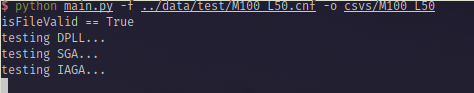
\includegraphics[scale=0.5]{img/single_run.png} \\
Przykładowe wywołanie programu $main.py$
\end{figure}

Wywołanie to przyjmuje nastepujące parametry:
\begin{itemize}
  \item f: plik z danymi w formacie DIMACS
  \item o: katalog docelowy dla plików wyjściowych w formacie csv
  \item i: liczba iteracji/wykonań pojedynczego algorytmu
\end{itemize}
\begin{figure}[h]
\centering
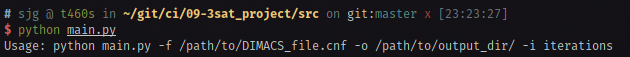
\includegraphics[scale=0.5]{img/help.png} \\
\end{figure}

Szereg wywołań programu $main.py$ stworzył poszczególne pliki opisujące wyniki pojedynczego eksperymentu.

\begin{figure}[h]
\centering
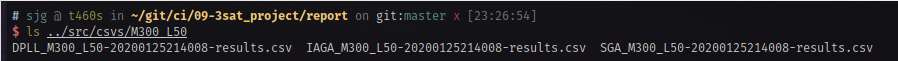
\includegraphics[scale=0.5]{img/csvdata.png} \\
\end{figure}

Przy użyciu zaimplementowanego skryptu $graph.py$ stworzono wykresy będące podstawą analizy wyników.\\
\textbf{Wykonanie algorytmów w wielu iteracjach pozwoliło na uśrednienie wyników pomiarów czasu zaprezentowanych na wykresach}
\pagebreak

\section{Wyniki}
\begin{figure}[h]
\centering
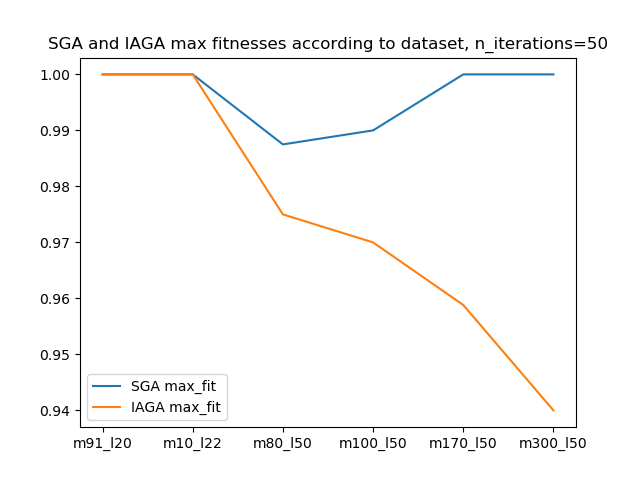
\includegraphics[scale=0.50]{img/plot2.png}
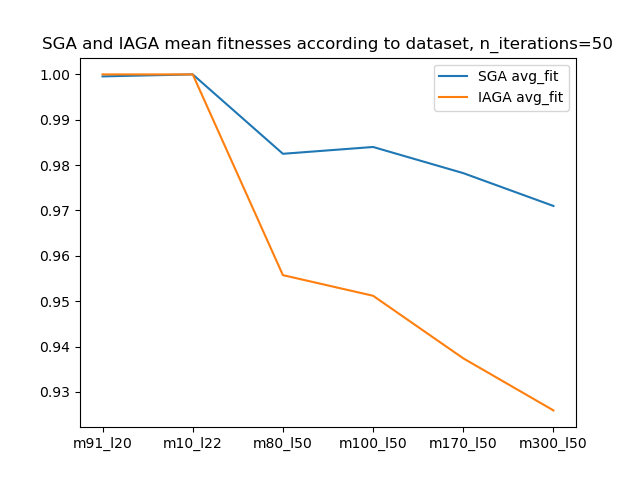
\includegraphics[scale=0.50]{img/plot3.png}
\end{figure}

\begin{figure}[h]
\centering
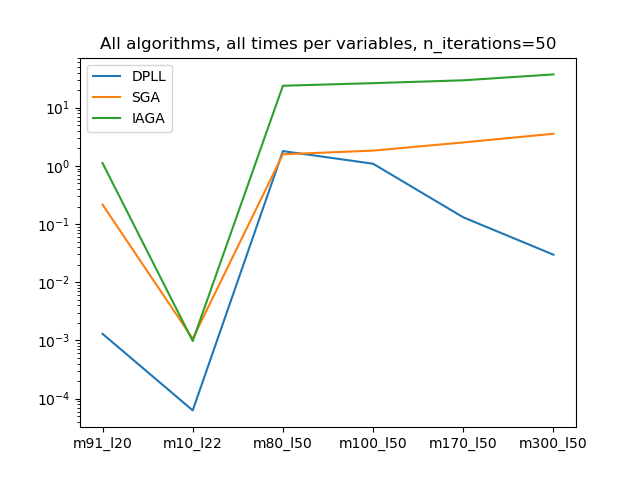
\includegraphics[scale=0.75]{img/plot1.png} \\
\end{figure}

\section{Interpretacja wyników}
\subsection{Wnioski}
\begin{enumerate}
  \item Zgodnie z oczekiwaniami algorytm \textbf{DPLL} zawsze gdy było to możliwe (dane wejściowe SAT) zwracał prawidłowe rozwiązanie w krótkim czasie
  \item Na czas wykonywania algorytmów wpływ ma nie tylko ilość klauzul ale również ilość zmiennych
  \item Zaimplementowany algorytm \textbf{SGA} okazał się równy bądź nawet lepszy od danych przedstawionych w \textit{An Improved Adaptive Genetic Algorithm for Solving 3-SAT Problems Based on Effective Restart and Greedy Strategy}
  \item Gdy algorytm \textbf{IAGA} nie był wstanie znaleźć spełnialnego rowiązania dla dużej ilości zmiennych $L >= 50$, bądź dla dużej ilości klauzul $M >= 150$ czas jego wykonania \textbf{rósł ze względu na ilość wykonywanych restartów}.
  \item Algorytm \textbf{IAGA} zwraca zdecydowanie więcej rozwiązań spełniających oraz zdecydowanie szybciej dla datasetu, który również jest spełnialny przez algorytm \textbf{SGA}.
  \item Zachodzi następująca prawidłowość: im mniejsza ilość zmiennych w problemie, tym krótszy czas wykonania algorytmu.
\end{enumerate}
\subsection{Możliwe błędy}
Niestety, publikacja naukowa, na której oparto implementacje algorytmu IAGA nie jest wystarczająco pełnowartościowa. Na szczególną uwagę zasługują niejasne rozdziały na temat zastosowanych strategii - w szczególności algorytm strategii wyboru oraz strategii zachłannej.\\
W związku z niewystarczającym opisem słownym, wymagane były eksperymentalne zaimplementowalnie strategii zachłannej na podstawie artykułu.
Jednym z przykładów może być podatność na występowanie dzielenia przez zero w opisie funkcji adaptycjnie liczącej współczynniki mutacji i rekombinacji.
\begin{figure}[h]
\centering
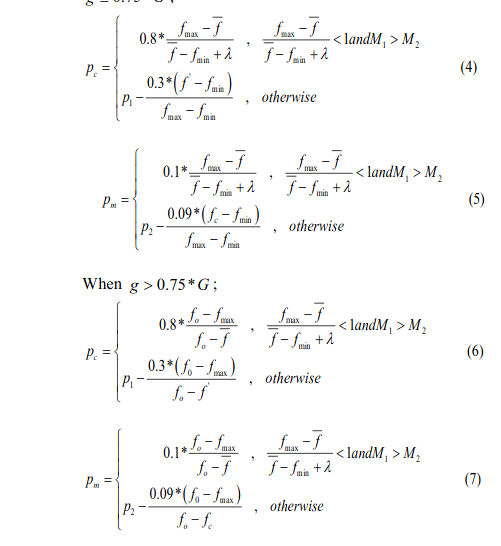
\includegraphics[scale=0.5]{img/lambda.png} \\
\end{figure}


%\begin{corollary}{1}
%
%\end{corollary}
\end{document}
